\section{Performance test}
This section contains the results from the performance test done by the subjects. First of the results from the regressor trained only with EMG data are presented, and afterwards compared to the regressor trained with inclusion of IMU data. The boxplot in \ref{fig:GotItTime} shows the test scores of all limb positions for both features.

\begin{figure}[H]
	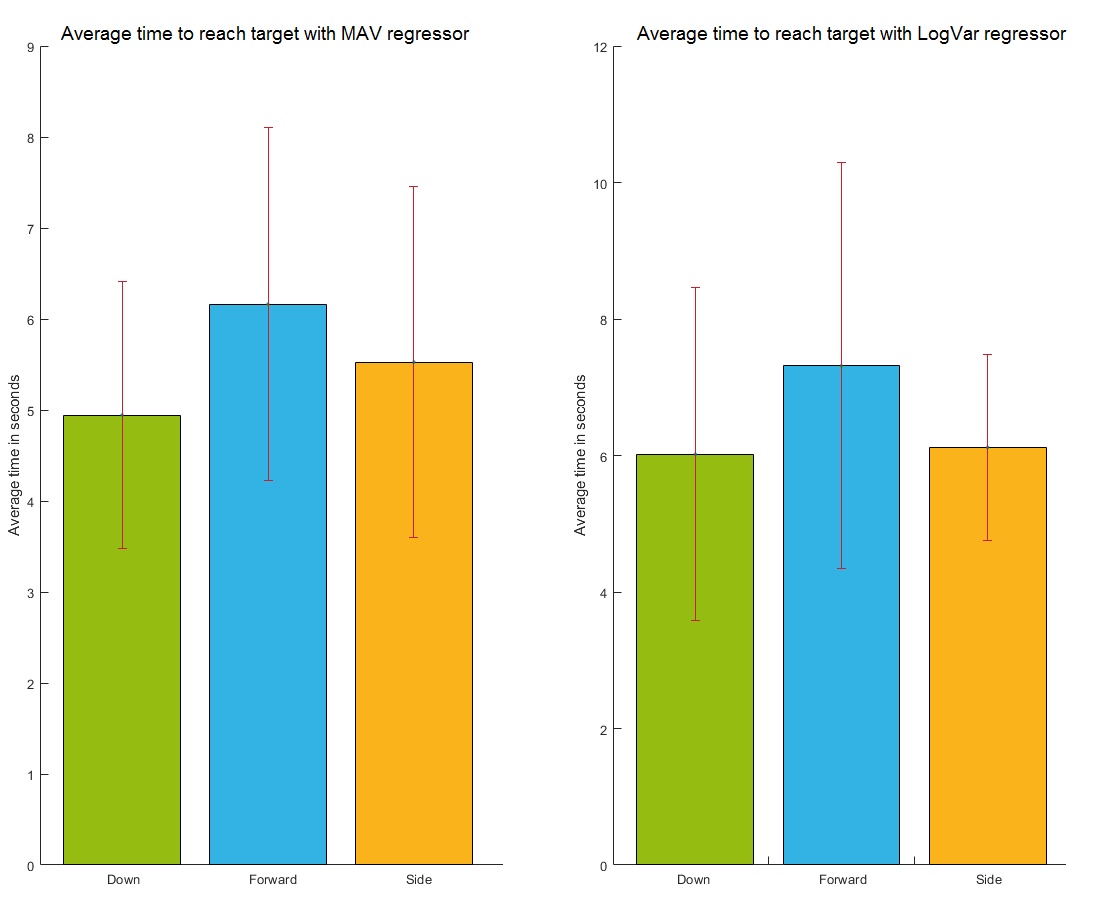
\includegraphics[width=0.7\textwidth]{figures/results/GotItTime}  %<--but is not needed.
	\caption{Calculated performance scores of the regressors trained with the logarithmic variance feature for the three limb positions. The bar chart illustrates the mean score across all subjects, and the error bar illustrates the standard deviation.}
	\label{fig:GotItTime}  %<--give the figure a label, so you can reference!
\end{figure}

A one-sample Kolmogorov-Smirnov test was done on the scores from the MAV and LogVar respectively and showed no normality in both score sets(p = $7 * 10^{-20}$, $8 * 10^{-20}$ ). A Friedman's test was therefore applied for statistical analysis. The performance scores between the three limb positions prove not to be significantly different (p = 0.57), when applying the LogVar trained regressors in the online test. For the MAV trained regressors the performance score between all limb positions can not be proven significantly different either(p = 0.16). When comparing all performance scores from the two feature trained regression control schemes, the Friedman's test proves no significant difference (LogVar: 6.5 s, MAC: 5.5 s; p = 0.13).

\begin{figure}[H]
	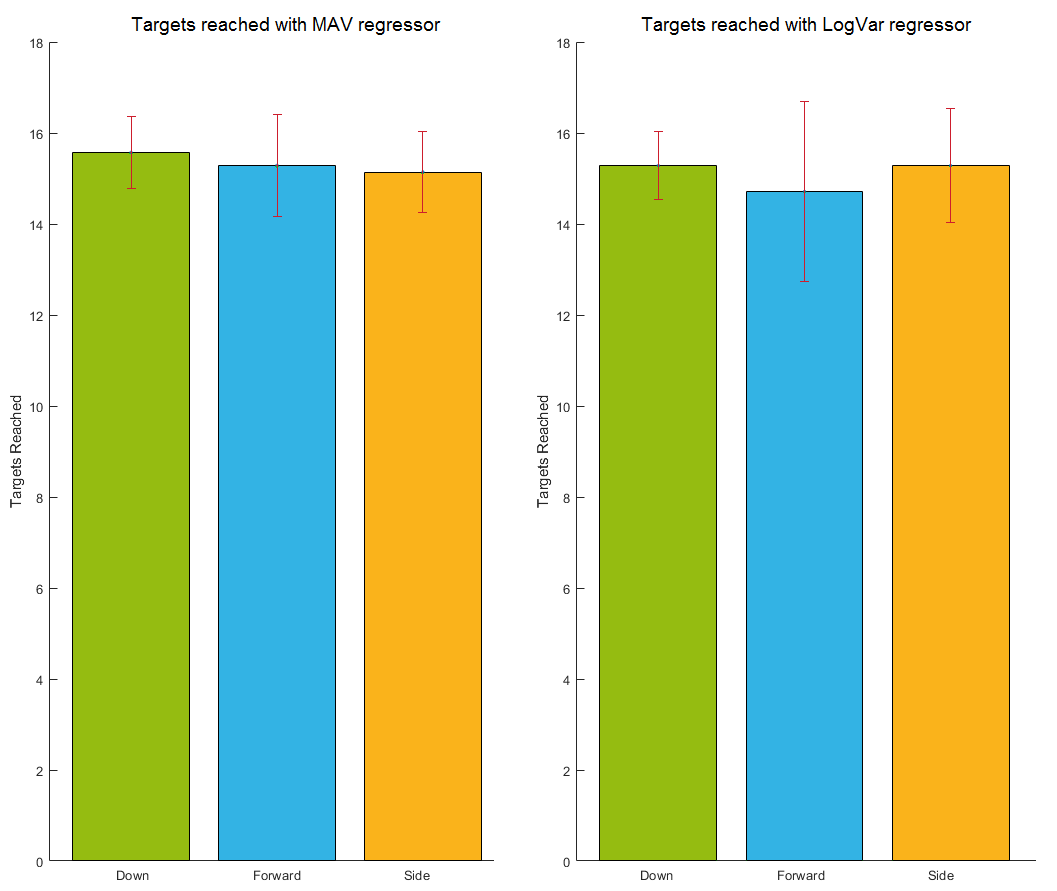
\includegraphics[width=0.7\textwidth]{figures/results/TargetsReached}  %<--but is not needed.
	\caption{The boxplot illustrates the amount of targets reached for the respective limb positions for both features.}
	\label{fig:TargetsReached}  %<--give the figure a label, so you can reference!
\end{figure}

A qualitative examination of the box plot in \ref{fig:TargetsReached} shows no significant difference in targets reached between limb positions and between all limb positions for the two features, which is similar to the Friedman's test results for the time per reached target.